% !TeX spellcheck = id_ID

%% isi proposal jika masih tahap proposal
%% isi skripsi jika sudah seminar proposal
\documentclass[skripsi]{skripsifasilkom}

%--------------------------------------------------
%Disini awal masukan untuk data proposal skripsi
%--------------------------------------------------

%isi nama lengkap, npm dan email
\namalengkap{Junaedi Fahmi}{1510631170081}{junaedi.fahmi15081@student.unsika.ac.id}



\judulindo{Penerapan \textit{Voice Verification} dan \textit{One Time Password} pada Otentikasi Mesin ATM}
\juduleng{The Implementation of Voice Verification and One Time Password in ATM Authentication System}


\tanggalseminar{19 Februari} %tanggal seminar proposal
\tanggalsidang{17 April} %tanggal sidang kolokium
\tahun{2019}

% ubah jika pimpinan berubah
\koprodi{Jajam Haerul Jaman, SE, M.Kom}{0010117808}
\dekan{Ade Andri Hendriadi, S.Si, M.Kom}{0402047903}

% untuk pembimbing nama lengkap, nidn, email
\pembimbingsatu{Nina Sulistiyowati, S.T, M.Kom}{0421108903}{nina.sulistio@staff.unsika.ac.id}

%pembimbing dua diisi ketika sudah mendapat SK
\pembimbingdua{Aji Primajaya, M.Kom}{0026048706}{aji.primajaya@staff.unsika.ac.id}

%penguji satu diisi saat masih tahap proposal
\pengujisatu{Penguji Satu}{00000000}

%penguji dua diisi saat akan sidang kolokium
\pengujidua{Pengujidua}{00000000}

%-----------------------------------------------------------------
%Disini akhir masukan untuk data proposal skripsi
%-----------------------------------------------------------------
\usepackage{lipsum}
\begin{document}

%% Diisi hanya jika menggunakan option skripsi %%
%--------------------------------------------%	
	\begin{persembahan}
		Untuk aku yang berjuang melawan diri sendiri,
	\end{persembahan}
	
	\begin{motto}
		Sucikanlah nama Tuhan mu Yang Maha Tinggi
	\end{motto}

	\begin{abstrak}
		\lipsum[1]	
		\katakunci{satu}
	\end{abstrak}

	\begin{abstract}
		\lipsum[1]
		\keywords{One Two}
	\end{abstract}
%%--------------------------------------------%


%%----------KATA PENGANTAR-------%%
\begin{katapengantar}
	\noindent
	Assalamu'alaikum Wr. Wb.
	
	Puji syukur penulis panjatkan ke hadirat Allah SWT karena dengan rahmat dan hidayah-Nya, Proposal Skripsi dengan judul "\textit{\textbf{Penerapan Voice Verification dan One Time Password pada Otentikasi Mesin ATM }}" ini dapat terselesaikan tanpa halangan berarti.
	
	Keberhasilan dalam menyusun proposal ini tidak lepas dari bantuan berbagai pihak yang mana dengan tulus dan ikhlas memberikan masukan guna sempurnanya proposal ini. Oleh karena itu dalam kesempatan ini, dengan kerendahan hati penulis mengucapkan terima kasih kepada:
	
	\begin{enumerate}
		\item Bapak Prof. Dr. H. Moh. Wahyudin Zarkasyi, SE, MS, Ak., CPA., selaku rektor Universitas Singaperbangsa Karawang.
		\item Bapak Ade Andri Hendriadi, S.Si, M. Kom selaku Dekan Fakultas Ilmu Komputer dan Dosen Wali penulis yang senantiasa memberikan motivasi.
		\item Bapak Aries Suharso, S.Si, M. Kom. selaku Wakil Dekan Fakultas Ilmu Komputer yang senantiasa mendampingi mahasiswa dalam proses pembuatan proposal skripsi ini.
		\item Bapak Jajam Haerul Jaman, S.E, M.Kom selaku Ketua Program Studi Teknik Informatika.
		\item Ibu Nina Sulistiyowati, S.T, M.Kom selaku dosen pembimbing yang selalu membimbing baik dalam penyusunan proposal ini maupun dalam hal lain.
		\item Dosen-dosen Fakultas Ilmu Komputer yang telah memberikan ilmu dan pelajaran hidup bagi penulis.
		\item Orang tua penulis, Kardi dan Irni Yuningsih yang selalu memberikan semangat dan kehidupan yang baik untuk penulis.
		\item Kawan seperjuangan Relawan TIK Karawang, yang setia menjadi guru bagi penulis.
	\end{enumerate}
	Penulis menyadari bahwa penyusunan proposal skripsi ini jauh dari sempurna. Akhir kata penulis mohon maaf yang sebesar-besarnya apabila ada kekeliruan di dalam penulisan proposal skripsi ini.

\begin{flushleft}
		Wassalamu'alaikum Wr. Wb.\\
\end{flushleft}
	\begin{tabular}{p{7.5cm}c}
		 & Karawang, 19 Februari 2019\\
		 &                           \\
		 &                           \\
		 &     \textbf{Penulis}
	\end{tabular} 
	%%------AKHIR KATA PENGANTAR-----%%
\end{katapengantar}	
	
	\pendahuluan
	%!TEX root = ./main.tex
\chapter{PENDAHULUAN}

\section{Latar Belakang}
	\lipsum
\section{Rumusan Masalah}
Berdasarkan latar belakang yang sudah dijelaskan, penulis merumuskan beberapa masalah dalam beberapa poin yang dapat dilihat di bawah ini,
\begin{enumerate}
\item Bagaimana membangun sistem otentikasi dua faktor (2FA) dengan menggabungkan faktor Biometrik berupa \textit{Voice Identification} dan \textit{One Time Password} ?
\item Bagaimana akurasi dari sistem dua faktor yang telah dibangun?
\item Bagaimana performa sistem yang telah dibuat?
\end{enumerate}

\section{Batasan Masalah}
Untuk menjaga pembahasan agar tetap fokus, maka penulis membatasi penelitian sebagai berikut:
\begin{enumerate}
	\item Implementasi sistem merupakan simulasi sistem otentikasi saja, bukan sistem ATM secara utuh.
	\item Implementasi sistem berbasis CLI (\textit{Command Line Interaction}) yang dibuat semirip mungkin dengan sistem ATM yang sudah ada.
	\item Sistem yang dibuat tidak menggunakan kartu ATM.
	\item Sistem yang dibuat hanya memiliki 20 orang nasabah, dengan komposisi 10 orang nasabah pria dan 10 orang nasabah wanita yang dipilih secara acak di sekitar lingkungan UNSIKA.
\end{enumerate}
\section{Tujuan Penelitian}
Tujuan dilakukan penelitian ini adalah sebagai berikut:
\begin{enumerate}
	\item Membangun sistem otentikasi dengan menggunakan OTP dan Voice Identification.
	\item Mengetahui akurasi dari sistem otentikasi yang dibuat.
	\item Mengetahui performa dari sistem otentikasi yang dibuat.
	\item Menguji skema otentikasi dengan menggunakan \textit{One Time Password} dan \textit{Voice Identification}
\end{enumerate}
\section{Manfaat Penelitian}
Penulis berharap dengan dilakukannya penelitian ini dapat memberikan manfaat-manfaat sebagai berikut.
\subsection{Manfaat Teoritis}
\begin{enumerate}
	\item Membuktikan akurasi sistem otentikasi dengan menggunakan multifaktor otentikasi.
	\item Memberikan pengetahuan mengenai akurasi dari penggunaan OTP dan Voice Identification dalam sistem otentikasi.
	\item Memperluas wawasan keilmuan dengan mengimplementasikan skema otentikasi yang berbeda.
\end{enumerate}
\subsection{Manfaat Praktis}
\begin{enumerate}
	\item Membantu penulis untuk mengimplementasikan keilmuannya pada masalah nyata.
	\item Memberikan rekomendasi untuk mengatasi penipuan yang dilakukan dengan menggunakan kartu ATM.
	\item Membantu Pemerintah dalam menjaga keamanan perekonomian mikro maupun makro.
\end{enumerate}

\section{Metodologi Penelitian}

Metodologi penelitian yang akan digunakan oleh penulis adalah metodologi penelitian eksperimen. 

\section{Sistematika Penulisan}
BAB I : PENDAHULUAN

Pada bab ini dijelaskan latar belakang, rumusan masalah, batasan, tujuan, manfaat, metodologi, sistematika penulisan serta jadwal penelitian.

BAB II : LANDASAN TEORI

Pada bab ini dijelaskan teori-teori dan penelitian terdahulu yang digunakan sebagai acuan dan dasar dalam penelitian.

BAB III : METODOLOGI PENELITIAN

Pada bab ini dijelaskan metode yang digunakan dalam penelitian meliputi langkah kerja, pertanyaan penelitian, objek penelitian dan alur penelitian .

\section{Jadwal Penelitian}

\begin{comment}
\bibliography{daftarpustaka}
\end{comment}
	%!TEX root = ./main.tex
\chapter{LANDASAN TEORI}

\section{Tinjauan Pustaka}
\subsection{Lorem}
\lipsum
\begin{tabel}[h]
	\caption{Apakah ini}
	\begin{tabular}{ccc}
		No & What & Ouh \\ \hline
		1 & ? & as
	\end{tabular}
\end{tabel}


%
\subsection{Mel Frequencies Cepstral Coefficients}
Salah satu teknik yang digunakan pada proses ektraksi fitur adalah Mel Factor Cepstral Coefficients (MFCC). \cite{Setiawan2011} menjelaskan, MFCC adalah proses pengubahan sinyal suara yang didasarkan pada variasi bandwidth kritis terhadap frekuensi yang dapat diterima telinga manusia yang berupa filter yang bekerja secara logaritmik pada frekuensi tinggi dan bekerja secara linear pada frekuensi tingkat rendah. Filter ini berguna untuk menangkap karakteristik fonetis yang penting dari sinyal gelombang suara. Untuk beradaptasi dengan kondisi telinga manusia, karakteristik ini digambarkan dalam skala mel-frekuensi yang berupa frekuensi linear di bawah 1000Hz dan frekuensi logaritmik di atas 1000Hz. Proses pengubahan data sinyal gelombang menjadi mffc dapat dilihat pada gambar di bawah ini:
\begin{figure}[H]
	\centering
	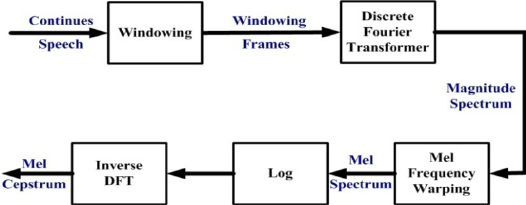
\includegraphics[width=0.7\linewidth]{Gambar/skema-mfcc}
	\caption{Alur kerja MFCC}
	\label{fig:skema-mfcc}
\end{figure}

\subsubsection{Frame Blocking}
Frame blocking adalah proses membagi sinyal gelombang suara yang panjang menjadi bagian-bagian kecil. Ucapan yang terdiri atas S sample $ X(S) $ dibagi menjadi beberapa frame yang berisi \textit{N} sample, masing-masing frame dipisahkan oleh M sample dengan $ M < N $. Frame pertama terdapat sampel \textit{N} pertama. Frame kedua dimulai \textit{M} sampel setelah permulaan frame pertama, sehingga frame pertama tumpang tindih (\textit{overlap}) dengan frame kedua sebanyak $ M-N $ sampel. Proses ini terus berlanjut hingga seluruh sampel berada dalam frame.
\subsubsection{Windowing}
Setelah proses frame blocking selesai dilakukan, proses windowing dilakukan agar meminimalkan diskontinuitas sinyal pada permulaan dan akhir setiap frame. Konsep windowing adalah meruncingkan sniyal mendekati angka nol pada permulaan dan akhir setiap frame. Jika window didefinisikan sebagai $ w(n), 0 \leq n \leq N-1s$ dengan N adalah jumlah sampel dalam tiap frame, maka hasil dari proses ini adalah gelombang:
\begin{equation}
y(n) = x(n) \cdot w(n), 0 \leq n \leq N -1
\end{equation}
dengan $y(n)$ = sinyal hasil \textit{windowing} ke-\textit{n}
$x(n)$ = nilai sampel ke-\textit{n}
$w(n)$ = nilai window ke-\textit{n}
\textit{N} = jumlah sampel dalam frame
Secara empirik penggunaan jenis window dalam mfcc adalah menggunakan hamming window dengan persamaan,
\begin{equation}
w(n) = 0.54 + 0.46 \cos \left( \frac{2\pi n}{N - 1} \right), 0 \leq n \leq N -1
\end{equation}

\subsubsection{Fast Fourier Transform}
Setelah dilakukan windowing dengan hamming window, langkah selanjutnya adalah mengubah sampel dari domain waktu ke domain frekuensi. Untuk melakukan ini kita akan mengimplementasi persamaan \textit{Discrete Fourier Transform} (DFT) ke dalam Fast Fourier Transform. Sampel yang sudah didapat kemudian dimasukkan ke dalam persamaan
\begin{equation}
f(n) =\sum_{k=0}^{N-1} y_{k} e^{-2\pi jkn / N}, n = 0,1,2, \ldots ,N-1
\end{equation}
\subsubsection{Mel-Frequency Wrapping}
Persepsi telinga manusia dalam freskuensi suara dalam sinyal ucapan tidak mengikuti skala linear. Maka, untuk setiap nada dengan frekuensi sesungguhnya \textit{f} dalam Hz, sebuah pola diukur dalam sebuah skala yang disebut 'mel'. Skala 'mel frekuensi' adalah skalan frekuensi linear di bawah 1000 Hz dan skala logaritmik di atas 1000 Hz.
Skala ini didefinisikan oleh %% cari paper tentang stanley smith 
sebagai :
\begin{equation}
mel(f) = 2595 \cdot \log_{10} \left(1 + \frac{f}{700}\right)
\end{equation}
Pendekatan yang mudah dipahami untuk simulasi spektrum dalam skala mel adalah dengan menggunakan \textit{filter bank}\label{idx:filbank} yang diletakan secara seragam dalam skala mel yang ditunjukkkan pada gambar di bawah ini:
\begin{figure}[H]
	\centering
	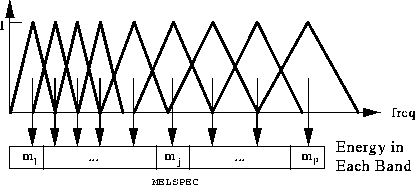
\includegraphics[width=0.7\linewidth]{Gambar/skala-mel}
	\caption{Skala Mel pada Filterbank}
	\figsource{Sumbernya dimana}
	\label{fig:skala-mel}
\end{figure}


Jika spektrum F[N] adalah masukan dalam proses ini, maka hasil proses ini adalah spektrum M[N] yang merupakan spektrum F[N] yang telah diubah dengan nilai berupa \textit{power output} dari filter-filter ini. Koefisien spektrum mel dinyatakan dalam K dan secara khusus ditentukan dengan nilai 20.
Dalam \textit{mel-frequency wrapping}, sinyal yang dihasilkan dalam proses sebelumnya dikelompokkan ke dalam berkas filter segitiga tersebut. Maksud dari pengelompokkan dalam hal ini adalah penjumlahan dari setiap nilai dari FFT dikalikan dengan\textit{gain filter} yang bersesuaian. Maka setiap kelompok memiliki sejumlah bobot energi sinyal yang ditampilkan sebagai $ m_1 \ldots m_p $ seperti dalam gambar.
\subsubsection{Cepstrum}
Ceptrum adalah istilah yang digunakan untuk kebalikan dari \textit{spectrum}. Untuk mendapatkan informasi dari sebuah suara yang diucapkan oleh manusia biasa menggunakan Ceptrum. Hasil dari proses \textit{mel-frequency wrapping} yang telah dilakukan, akan dikonvesi menggunakan \textit{Discrete Cosine Transform} (DCT) untuk mendapatkan nilai dari Mel-Frequency Ceptrum Coefficients (MFCC).
Secara formal MFCC didefinisikan sebagai alihragam kosinus dari logaritma \textit{short-term power spectrum} yang dinyatakan dalam skala mel-frekuensi. Jika $S_k, k = 1,2, \ldots, K$ dinyatakan sebagai \textit{mel power spectrum coefficients}, Minh N.Do mendefinikan koefisien dari MFCC sebagai:
\begin{equation}
c_n = \sum_{k=1}^{K} (log S_k) \cos\left[ n(k- \frac{1}{2}) \frac{\pi}{K} \right] , n = 1,2, \ldots ,K
\end{equation}


\subsection{i-Vector}
i-Vector Extraction atau ekstraksi i-vector adalah sistem yang memproyeksikan sekuens dari vektor (biasanya cepstral coeffiecients) yang diperoleh dari ucapan, $ O = \lbrace o_t\rbrace_{t=1}^{N} $ dengan $ o_t \in \mathbf{R}^F $, ke dalam vektor dengan panjang tertentu $ \eta \in \mathbf{R}^D $. Untuk melakukan itu, sebuah Gaussian Mixture Model dengan K komponen , $ \lambda = ( \lbrace w_k \rbrace, \lbrace m_k \rbrace,\lbrace \Sigma_k \rbrace) $ yang didenotasikan sebagai Universal Background Model (UBM) digunakan untuk mengambil Baum-Welch statistik dari setiap ucapan. Selanjutnya, sebuah supervector $ \theta = [ \theta_1^T, \ldots,  \theta_K^T]^T \in \mathbf{R}^{FK}$ dibangun dengan cara menyatukan statistik tingkat pertama dari masing-masing komponen \textit{mixture} dengan asumsi mengikuti persamaan model linear standard dalam bentuk:
\begin{equation}
\theta = m+\mathtt{T}x 
\end{equation}
dimana, supervector $ m \in \mathbf{R}^{FK} $ diperoleh dari UBM, $ T \in \mathbf{R}^{FK \times D}$ berupa matriks dari kolom-kolom rank rendah yang diperluas dalam subruang dimana kebanyakan informasi khas dari masing-masing pembicara, dan  sebagai variabel laten dari distribusi normal. Untuk setiap ucapan, i-vector $\eta$ diperoleh sebagai peta dari  perkiraan posisi dari. Subruang yang diperluas oleh  diperoleh dari himpunan data representatif yang besar  dari proses estimasi yang dilakukan oleh Machine Learning.
\subsection{One Time Password}


\newpage
\section{Penelitian Sebelumnya}
\begin{enumerate}
	
	\item Penulis: Jos\`{e} Port\^{e}lo, Bhiksha Raj, Alberto Abad dan Isabel Trancoso\\ 
	Tahun: 2014\\
	Judul: \textit{Privacy-Preserving Speaker Verification using Secure Binary Embedding}  \\
	\lipsum[1]
	
	\item Penulis: Lee Mun Kyu, Nam Hyeongjin dan Kim Dong Kyu\\
	Tahun: 2017\\
	Judul: \textit{Secure Biomodal PIN-Entry Method using audio signals}  \\
	\lipsum[2]
	
	\item Penulis : Reshma Begum, Basavaraj Gadgay, Veeresh Pujari, Pallvi B. V. \\
	Tahun : 2017 \\
	Judul : \textit{Security of ATM System Using Biometric and OTP}
	\lipsum[3]
	
	\item Penulis : Aleluya dan Vicente\\
	Tahun : 2018 \\
	Judul : \textit{FacetureID: face and hand gesture multi-factor authentication using deep learning.}\\
	\lipsum[4]
	
	\item Penulis : Junaedi Fahmi\\
	Tahun: 2018\\
	Judul : Pengunaan \LaTeX untuk mengurangi kegalauan skripsi\\
	\lipsum[5]
\end{enumerate}

\begin{penelitianterkait}
	\captionof{table}{Perbedaan Penelitian }
	\begin{longtable}{|p{0.5cm} | p{3.2cm} | p{3.2cm} | p{7cm} | p{7cm} | }
		\hline
		\thead{No} & \thead{Penulis (Tahun)} & \thead{Judul} & \thead{Hasil} & \thead{Keterangan} \\ \hline
		1          &                         &               &               &                    \\ \hline
		2          &                         &               &               &                    \\ \hline
		3          &                         &               &               &                    \\ \hline
		4          &                         &               &               &                    \\ \hline
		5          &                         &               &               &                    \\ \hline
	\end{longtable}
\end{penelitianterkait}

\subsection{Penelitian Sekarang}

Penelitian sekarang adalah menguji skema otentikasi menggunakan dua faktor. Faktor pertama dengan menggunakan OTP dan faktor kedua dengan biometrik. Biometrik yang digunakan berupa suara. Proses verifikasi menggunakan suara menggunakan teknologi Jaringan Saraf Tiruan dengan topologi yang disesuaikan.

\begin{comment}
\bibliography{daftarpustaka}
\end{comment}
	%!TEX root = main.tex
\chapter{OBJEK DAN METODOLOGI PENELITIAN}

\section{Objek Penelitian}

Objek yang akan menjadi bahan kajian pada penelitian ini adalah sistem otentikasi atau sistem login pada mesin ATM. Sistem otentikasi pada mesin ATM yang ada sekarang menggunakan kartu dan PIN sebagai alat otentikasinya.

Proses otentikasi yang dilakukan sekarang adalah dengan memasukkan kartu ATM kedalam mesin kemudian mesin akan meminta otentikasi berupa PIN yang akan dimasukkan oleh pengguna melalui tombol yang ada pada mesin.

%Perangkat berupa mesin elektronik yang terhubung dengan pusat komputer layanan nasabah pada suatu lembaga penyimpan dana, sehingga dapat menggantikan sebagian fungsi kasir. Perangkat tersebut akan memungkinkan nasabah untuk melakukan transaksi dengan menggunakan suatu media baik berupa kartu atau media lainnya sebagai suatu identitas pengenal di dalam sistem. Jenis transaksi yang umum dilakukan melalui ATM antara lain berupa penarikan uang tunai dari rekening simpanan, pengecekan saldo, transfer kepada bank yang sama atau bank yang lain, serta pembayaran/pembelian berbagai barang/jasa.

\section{Metodologi Penelitian}

Metode pengembangan yang digunakan pada penelitian ini adalah metodologi standard pada pengembangan aplikasi yang menggunakan ekplorasi data yaitu \textit{CRoss InduStry Process for Data Mining} (CRISP-DM). CRIPS-DM digunakan karena kemampuan metologi tersebut yang dapat diterapkan kepada hampir semua jenis bisnis. Ada enam fase yang ada dalam metodologi ini yaitu \textit{Business Understanding}, \textit{Data Understanding},\textit{Data Preparation}, \textit{Modeling}, \textit{Evaluation} dan \textit{Deployment}.

\begin{figure}[h]
	\centering
	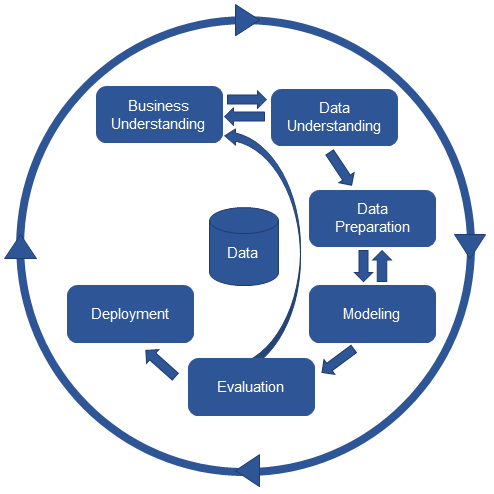
\includegraphics[width=0.7\linewidth]{Gambar/crisp-dm}
	\caption{Fase-fase pada CRIPS-DM}
	\label{fig:crisp-dm}
\end{figure}


\newpage
\section{Rancangan Penelitan}

Rencana penelitian yang akan dilaksanakan adalah sebagai berikut:
\begin{figure}[H]
	\centering
	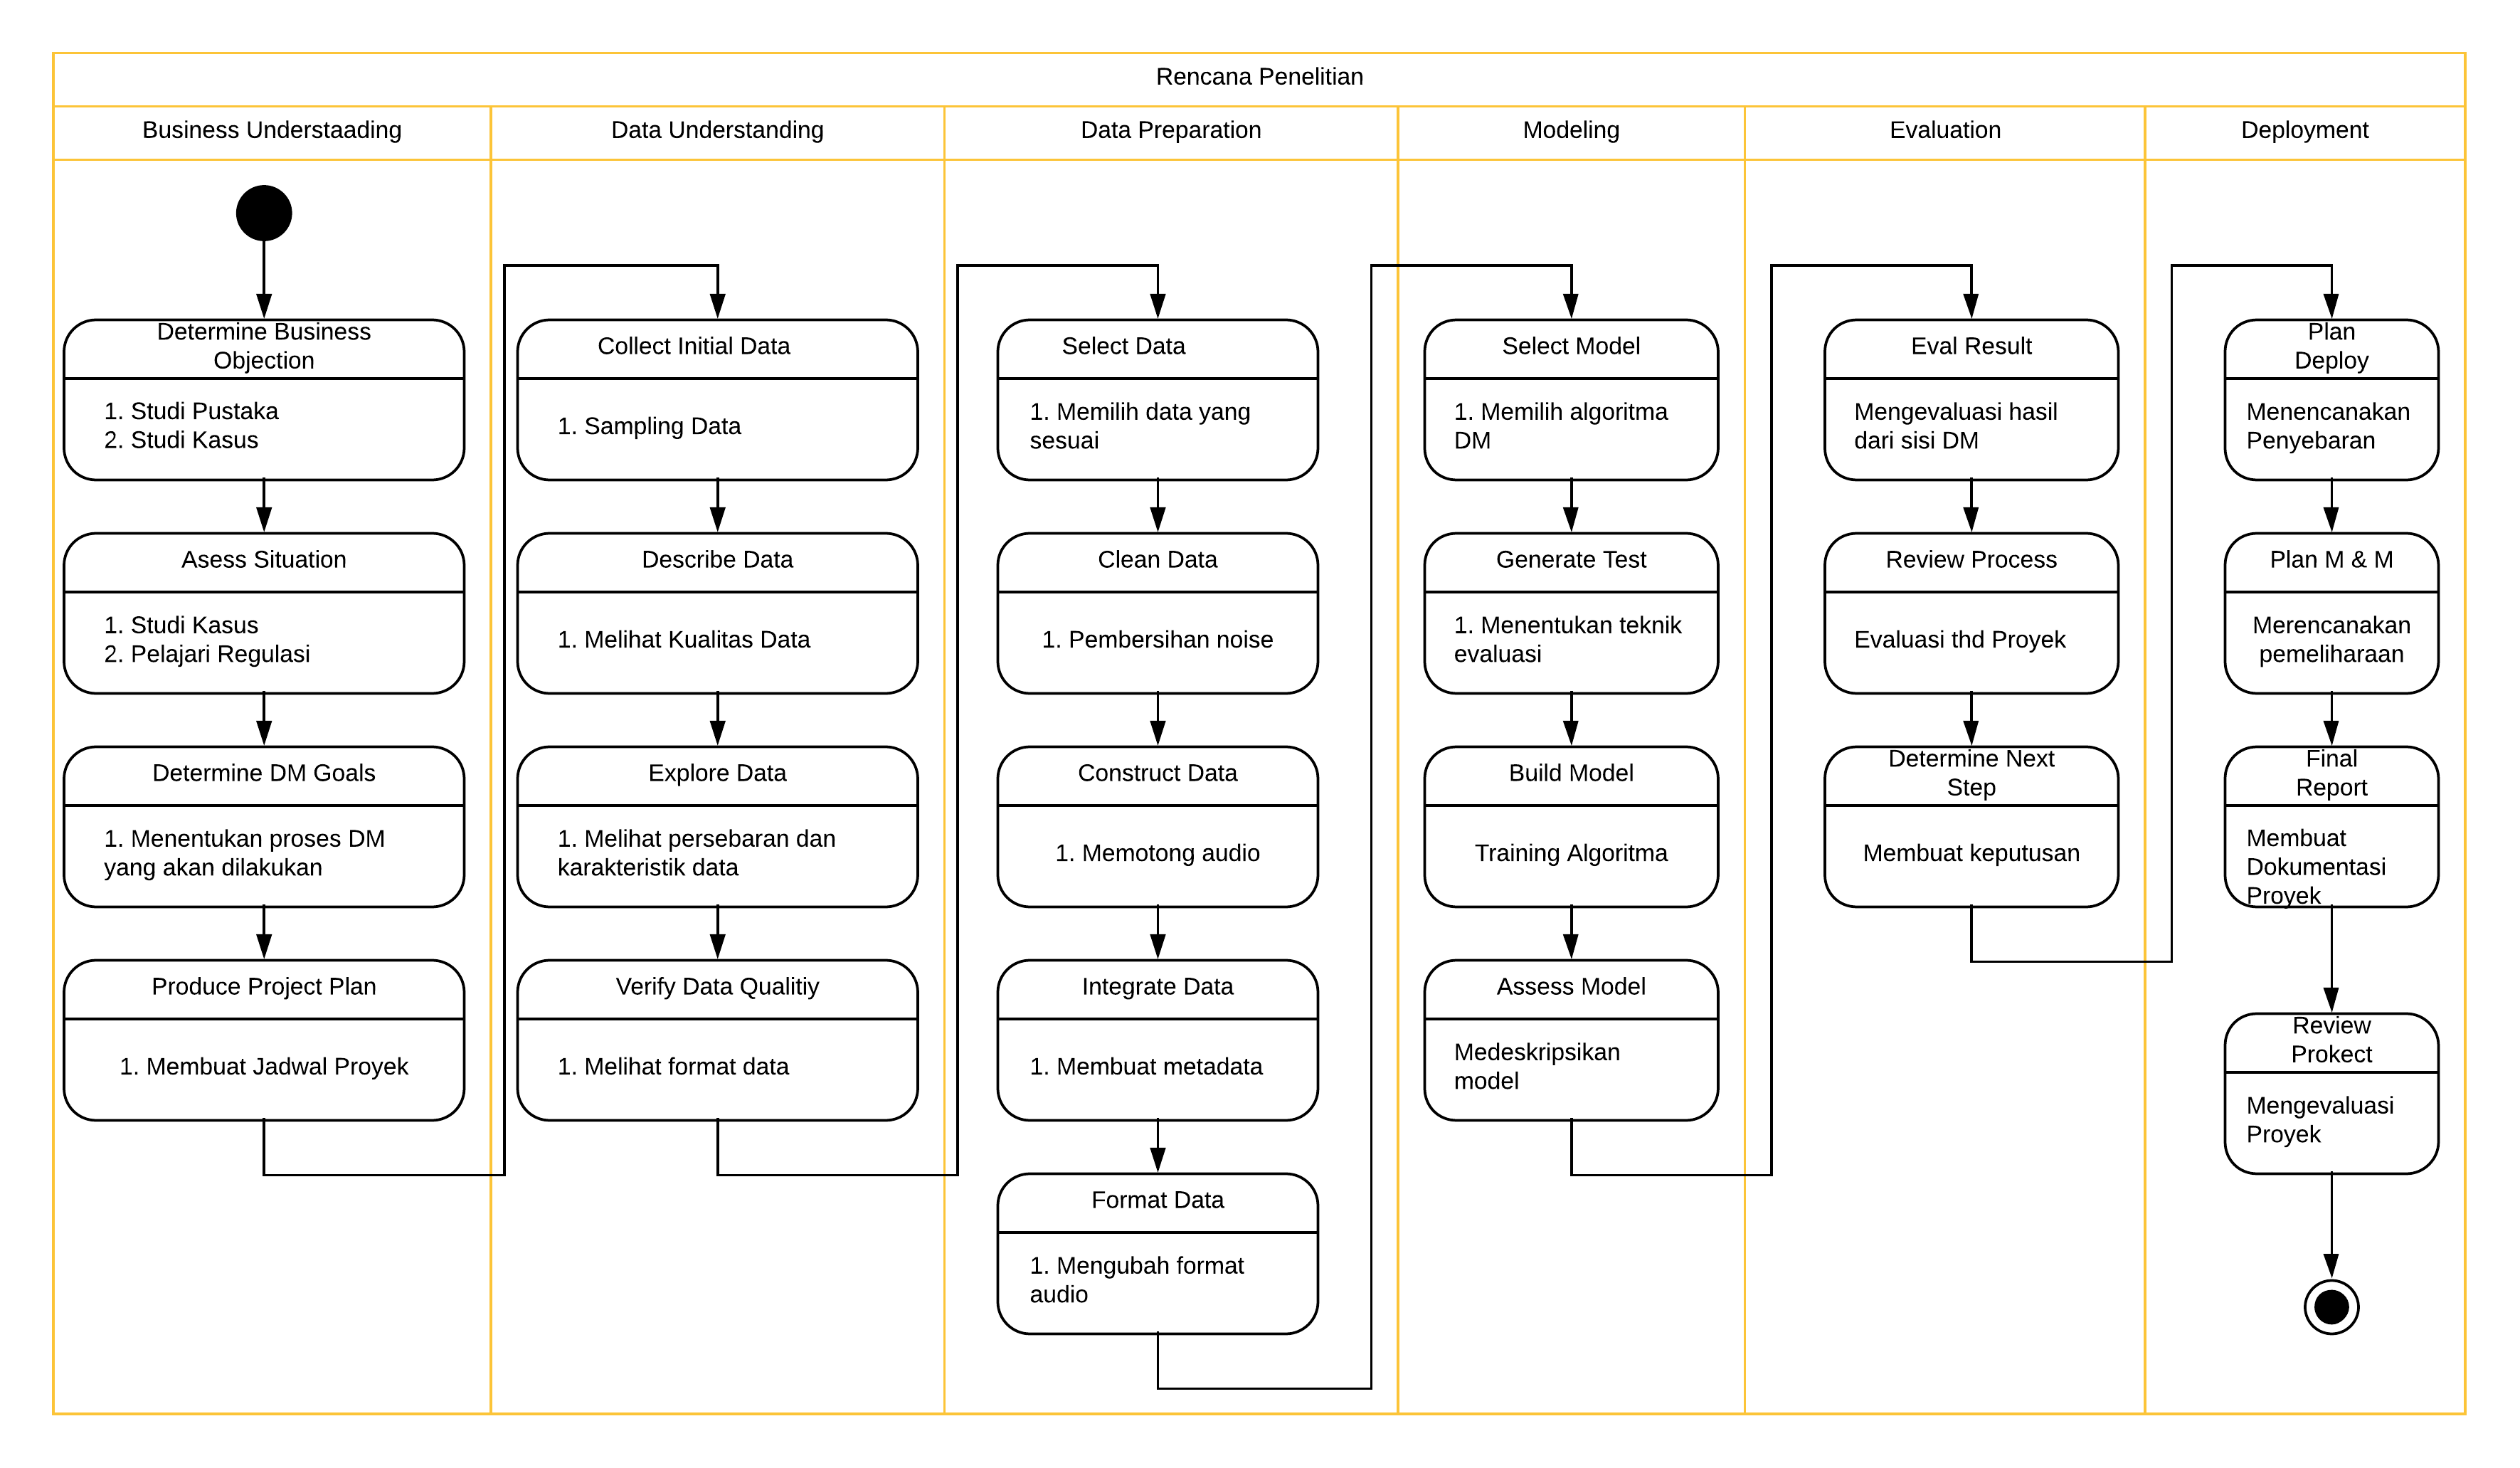
\includegraphics[width=1\linewidth]{Gambar/rencana-penelitian}
	\caption{Rencana Penelitian}
	\label{fig:rencana-penelitian}
\end{figure}


\begin{enumerate}
	\item \textit{Business Understanding}\\
	Pada fase ini, akan dilakukan studi pustaka mengenai objek penelitian yang akan diteliti. Perbandingan penerapan sistem serupa juga yang telah diterapkan di beberapa bagian dunia juga akan dikaji sebagai perbandingan. Beberapa kasus penyalahgunaan identitas juga dikaji sehingga solusi yang ditawarkan diharapkan menjadi efektif. Proses \textit{data mining}  ditawarkan sebagai solusi dengan tujuan untuk menyelesaikan permasalahan yang telah dikemukakan. Beberapa kriteria keberhasilan juga ditentukan di fase ini.
	\item \textit{Data Understanding}\\
	Di fase ini dilakukan pengumpulan data awal sebagai tolok ukur kualitas data. Pada fase ini akan dilakukan pengumpulan data suara dari 20 orang responden yang dipilih menggunakan metode sampling \textit{stratified-sampling}. Metode\textit{ stratified-sampling} adalah metode pengumpulan data dengan cara membagi populasi ke dalam sub-populasi dan mengambil sejumlah sampel dari masing-masing sub populasi tersebut. Pada penelitian ini, akan dilakukan pengambilan data dengan cara merekam suara responden dengan menggunakan perangkat telepon genggam. Masing-masing responden akan diminta untuk mengucapkan angka 0 s.d. 9 sebanyak tiga kali. Responden akan diambil dari mahasiswa dan/atau dosen di lingkungan Fakultas Ilmu Komputer dengan komposisi 10 orang laki-laki dan 10 orang perempuan.
	
	\item \textit{Data Preparation}\\
	Setelah fase sebelumnya dilakukan, maka data suara yang telah dikumpulkan akan dibersihkan dan disamakan format data dari masing-masing berkas suara. Setiap berkas suara yang ada akan dilakukan formating dengan aturan sebagai berikut:
	\begin{table}[H]\label{tbl:formatdata}
		\vspace{-2em}
		\centering
		\footnotesize
		\singlespacing
		\caption{Format Data}
		\begin{tabular}{|c|l|r|}
			\hline
			\thead{No} & \thead{Atribut} & \thead{Format} \\ \hline
			1 & Format File & WAV \\ \hline
			2 & Sample Rate & 22050 Hz \\ \hline
			3 & Bit Rate & 16 bit \\ \hline
			4 & Nama File & uuid \\ \hline
			5 & Panjang Suara & 1000 ms \\ \hline
		\end{tabular}
	\vspace{-2em}
	\end{table}
	
	Proses ini dapat dilakukan dengan menggunakan aplikasi ffmpeg. Kemudian data tersebut dibagi menjadi data uji dan data latih dengan perbangingan 20:80. Luaran dari fase ini adalah sebuah metadata yang memetakan file suara dengan pembicara yang bersesuaian. 
	
	\item \textit{Modeling}\\
	Fase ini adalah fase membuatan model dari data yang sudah dimiliki. Fase ini termasuk didalamnya proses \textit{Feature Engineering} dan \textit{Model Building}.
	Proses \textit{Feature Engineering} akan dilakukan dengan menggunakan metode MFCC dengan jumlah koefisien yang dapat divariasikan sesuai dengan kebutuhan. Selanjutnya proses pelatihan model akan dilakukan dengan melatih model dengan menggunakan data latih yang telah ditentukan sebelumnya. Model data mining yang digunakan pada proses ini adalah model \textit{Multilayer Perceptron} dengan arsitektur yang digunakan dapat diubah sesuai hasil pelatihan.
	
	\item \textit{Evaluation}\\
	Pada fase ini dilakukan pengujian dari model yang telah dibangun di proses sebelumnya. Teknik pengujian yang digunakan pada model menggunakan \textit{False Rejected Rate}, \textit{False Acceptance Rate} dan Akurasi. Pengujian tersebut dilakukan dengan cara menggunakan model untuk memprediski data uji yang sudah disiapkan. Jika hasil yang diperoleh sudah memenuhi kriteria kesuksesan, maka dapat dilakukan fase terakhir.
	
	\item \textit{Deployment}\\
	Terakhir, fase deployment akan dilakukan dengan cara membangun aplikasi simulasi dengan menggunakan bahasa pemrograman Python. Pada fase ini juga dilakukan penggabungan dengan teknik OTP yang sudah disiapkan sebelumnya. Pengujian sistem pada fase ini adalah Unit Test dengan bantuan dari module unittest dari bahasa python.
\end{enumerate}

\begin{comment}
\bibliography{daftarpustaka}
\end{comment}
	
%% Jika sudah melaksanakan seminar proposal ini di uncoment
	%!TEX root = main.tex
\chapter{HASIL DAN PEMBAHASAN}

\section{Hasil}
\lipsum
\section{Pembahasan}
\lipsum
\lipsum

\begin{tabel}
	\begin{tabular}{|c|c|c|}
		\hline
		no & more & you\\ \hline
		Ai &  love & yu \\
		Ai &  love & yu \\
		Ai &  love & yu \\
		Ai &  love & yu \\\hline
	\end{tabular}
\end{tabel}
	%!TEX root = main.tex
\chapter{PENUTUP}
\section{Kesimpulan}
Berdasarkan penelitian yang telah dilakukan, maka didapatkan kesimpulan sebagai berikut:
\begin{enumerate}
	\item 
\end{enumerate}
\section{Saran}
%%----------------------------------------------------------


	\singlespacing
	\bibliography{daftarpustaka}
	\addcontentsline{toc}{chapter}{DAFTAR PUSTAKA}

	
%ketika pilih option skripsi ini di uncomment
 %!TEX root=./skripsi_fasilkom.tex

\begin{lampiran}{Data Diri}
	% \includepdf[pages=1]{bimbingan}
\end{lampiran}

\begin{lampiran}{Scan Kartu Bimbingan}
	content...
\end{lampiran}

\begin{lampiran}{Source Code}
	content...
\end{lampiran}
	
	
\end{document}